\documentclass[a4paper,oneside,12pt]{book}

% KODOVANI, CESTINA
\usepackage[utf8]{inputenc}
\usepackage[czech]{babel}
\usepackage{graphicx}
\usepackage{subcaption}

\DeclareGraphicsRule{*}{mps}{*}{}

% MATEMATIKA, CITACE, ...
\usepackage{amsthm}
\usepackage{amssymb}
\usepackage{enumerate}
\usepackage{hyperref}
\usepackage{cite}
\usepackage{amsmath}

% ODKAZY
\usepackage{hyperref}

% DEFINICNI BLOK
\theoremstyle{definition}
\newtheorem{df}{Definice}
\newtheorem*{zn}{Značení}
\newtheorem*{pr}{Příklad}

\theoremstyle{plain}
\newtheorem{vt}{Věta}
\newtheorem*{tv}{Tvrzení}
\newtheorem*{pz}{Pozorování}
\newtheorem{lm}{Lemma}
\newtheorem*{hp}{Hypotéza}

\theoremstyle{remark}
\newtheorem{po}{Poznámka}

%--------------------------------------------------

\begin{document}

% ---------------------------------- Obsah ----------------------------------- %
\tableofcontents

\setcounter{page}{1}

\pagebreak


% ----------------------------------- Úvod ----------------------------------- %
{
  \pagestyle{plain}
  
  \chapter*{Úvod}
\addcontentsline{toc}{chapter}{Úvod}

Matematické programování (optimalizace) se zabývá hledáním optimálních řešení matematických modelů. Modely, ve kterých se vyskytují pouze lineární funkce se zabývá lineární programování. Začátky lineárního programování jsou spojeny s druhou světovou válkou. George Dantzig, který měl na starosti vývoj logistických plánu na straně amerického letectva, v roce 1947 vymyslel Simplexovou metodu. S podobným konceptem přišel už dříve v~roce 1939 Leonid Kantorovič, ale na jeho práci bohužel nikdo nenavázal. Další slavná jména, která stojí za zmínku v souvislosti s lineárním programováním jsou John von Neumann, Albert Tucker, Harold Kuhn a spousta dalších. Relativně nová oblast optimalizace se nazývá semidefinitní programování, kterou dobře charakterizuje název článku z roku 1981 s názvem \textit{Linear Programming with Matrix Variables} od Cravena a Monda. Pokud máme optimalizační problém, ve kterém řešení jsou vyjádřena pomocí diskrétních proměnných, pak hovoříme o problému kombinatorické optimalizace. K řešení těchto problémů se v posledních cca 30 letech rozšířilo semidefinitní programování, které se využívá např. u Shannonovy kapacity grafu, studia řezů, problému obchodního cestujícího a dalších. Pro další historické informace související s optimalizací doporučuji zdroj \cite{history}, ze kterého bylo čerpáno.
  
  \clearpage
}


% ------------------------ ČÁST: KONVEXNÍ OPTIMALIZACE------------------------ %
\part{Konvexní optimalizace}

\chapter{Základní geometrické pojmy}

\section{Přímky a úsečky}

Mějme dva body $x_1, x_2 \in \mathbb{R}^n$ takové, že $x_1 \neq x_2$ a parametr $\theta \in \mathbb{R}^n$. Potom výraz
\begin{equation}
    y = \theta x_1 + (1 - \theta) x_2
    \label{line}
\end{equation}
popisuje \textbf{přímku} procházející body $x_1$ a $x_2$. Pro $\theta = 0$ dostáváme bod $x_2$ a pro $\theta = 1$ bod $x_1$. Omezíme-li $\theta$ na interval $\langle 0, 1 \rangle$, dostaneme \textbf{úsečku} s koncovými body $x_1$ a $x_2$. Výraz \ref{line} lze přepsat do tvaru
$$
    y = x_2 + \theta (x_1 - x_2),
$$
který můžeme interpretovat jako součet počátečního bodu $x_2$ a nějakého násobku směrového vektoru $x_1 - x_2$.

\section{Afinní prostory}

Říkáme, že $C \subseteq \mathbb{R}^n$ je \textbf{afinní prostor}, jestliže přímka procházející libovolnými dvěma různými body z $C$ leží v $C$. Tedy $C$ obsahuje lineární kombinace libovolných dvou bodů z $C$, jestliže součet koeficientů lineární kombinace je roven jedné. To lze zobecnit i pro více než dva body. Lineární kombinace $\theta_1 x_1 + \dots + \theta_k x_k$ bodů $x_1, \dots, x_k$ taková, že $\theta_1 + \dots + \theta_k = 1$, se nazývá \textbf{afinní kombinace} bodů $x_1, \dots, x_k$. Indukcí z definice afinního prostoru lze snadno ukázat, že pokud $C$ je afinní množina, $x_1, \dots, x_k \in C$ a $\theta_1 + \dots + \theta_k = 1$, potom bod $\theta_1 x_1 + \dots + \theta_k x_k \in C$.

\noindent Nechť $C$ je afinní prostor a $x_0 \in C$, potom množina
$$
    V = C - x_0 = \left\{ x - x_0 \mid c \in C \right\}
$$
je \textbf{vektorový prostor}, tj. množina, která je uzavřená na sčítání a násobení skalárem.

\noindent Afinní prostor $C$ lze vyjádřit jako
$$
    C = V + x_0 = \left\{ v + x_0 \mid v \in V \right\},
$$
kde $V$ je vektorový prostor a $x_0$ je počátek. Poznamenejme, že vektorový prostor $V$ asociovaný s afinním prostorem $C$ nezávisí na volbě počátku $x_0$.

\noindent \textbf{Dimenze} afinního prostoru $C = V + x_0$ je definována jako dimenze vektorového prostoru $V = C - x_0$, kde $x_0$ je libovolný prvek z $C$. Množina všech afinních kombinací bodů množiny $C \subseteq \mathbb{R}^n$ se nazývá \textbf{afinní obal} množiny $C$. Afinní obal množiny $C$ budeme značit
$$
    \textbf{aff } C = \left\{ \theta_1 x_1 + \dots + \theta_k x_k \mid x_1, \dots, x_k \in C, \theta_1 + \dots + \theta_k = 1 \right\}.
$$
Afinní obal je nejmenší afinní prostor, který obsahuje množinu $C$. Tedy, jestliže $S$ je afinní prostor takový, že $C \subseteq S$, potom $\textbf{aff }C \subseteq S$.


\section{Konvexní množiny}

Říkáme, že množina $C$ je \textbf{konvexní}, jestliže úsečka mezi libovolnými dvěma body z $C$ leží také v $C$. Jinak řečeno, jestliže pro libovolné dva body $x_1, x_2 \in C$ a libovolné $\theta \in \langle 0, 1 \rangle$ platí, že $\theta x_1 + (1 - \theta) x_2 \in C$. Poznamenejme, že každý afinní prostor je zároveň konvexní množinou. Podobně jako afinní kombinaci definujeme \textbf{konvexní kombinaci} bodů $x_1, \dots, x_k$ jako $\theta_1 x_1 + \dots + \theta_k x_k$, kde $\theta_1 + \dots + \theta_k = 1, \theta_i \geq 0$ pro $i = 1, \dots, k$. \textbf{Konvexní obal} množiny $C$ je množina všech konvexních kombinací bodů z množiny $C$, značíme
$$
    \textbf{conv }C = \left\{ \theta_1 x_1 + \dots + \theta_k x_k \mid x_i \in C, \theta_i \geq 0, i = 1, \dots, k, \theta_1 + \dots + \theta_k = 1 \right\}.
$$
Analogicky, konvexní obal množiny $C$ je nejmenší konvexní množina, která obsahuje množinu $C$. Pro představu viz obrázek~\ref{fig:convex_hull}.

\begin{figure}[h!]
    \centering
    \begin{subfigure}[b]{0.3\textwidth}
        \centering
        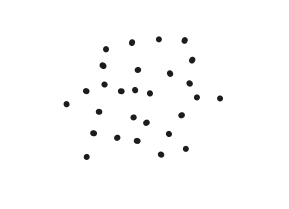
\includegraphics[width=\textwidth]{img/points_for_convex_hull.png}
        \caption{Množina bodů $C$}
        \label{fig:convex_hull:a}
    \end{subfigure}

    \hfill

    \begin{subfigure}[b]{0.3\textwidth}
        \centering
        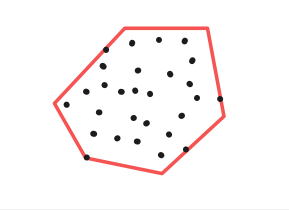
\includegraphics[width=\textwidth]{img/convex_hull.png}
        \caption{$\textbf{conv }C$}
        \label{fig:convex_hull:b}
    \end{subfigure}
     
    \caption{Konvexní obal množiny}
    \label{fig:convex_hull}
\end{figure}


\section{Kužely}

Množina $C$ se nazývá \textbf{kužel}, jestliže pro každé $x \in C$ a $\theta \geq 0$ platí, že $\theta x \in C$. Je-li $C$ navíc konvexní, pak se $C$ nazývá \textbf{konvexní kužel}. Tedy $C$ je konvexní kužel, jestliže pro libovolné $x_1, x_2 \in C$ a $\theta_1, \theta_2 \geq 0$ platí, že $\theta_1 x_1 + \theta_2 x_2 \in C$. Říkáme, že bod ve tvaru $\theta_1 x_1 + \dots + \theta_k x_k$, kde $\theta_1, \dots, \theta_k \geq 0$ je \textbf{kuželovou kombinací} bodů $x_1, \dots, x_k$. Dále, pokud $x_i$ leží v konvexním kuželu množiny $C$, potom libovolná kuželová kombinace bodu $x_i$ leží rovněž v konvexním kuželu množiny $C$. Platí, že množina $C$ je konvexní kužel právě tehdy, když $C$ obsahuje všechny kuželové kombinace svých bodů. \textbf{Kuželový obal} množiny $C$ je množina, která obsahuje všechny kuželové kombinace množiny $C$, tj.
$$
    \textbf{cone }C = \left\{ \theta_1 x_1 + \dots + \theta_k x_k \mid x_i \in C, \theta_i \geq 0, i = 1, \dots, k \right\}.
$$
Kuželový obal množiny $C$ je zároveň nejmenší konvexní kužel, který obsahuje množinu $C$. Pro představu viz obrázek~\ref{fig:cone_hull}.

\begin{figure}[h!]
    \centering
    \begin{subfigure}[b]{0.3\textwidth}
        \centering
        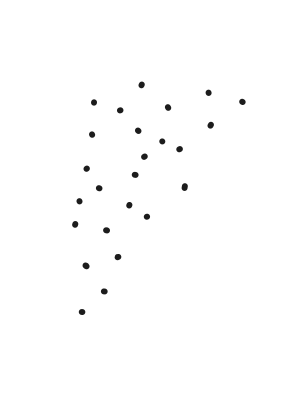
\includegraphics[width=\textwidth]{img/points_for_cone_hull.png}
        \caption{Množina bodů $C$}
        \label{fig:cone_hull:a}
    \end{subfigure}

    \hfill

    \begin{subfigure}[b]{0.3\textwidth}
        \centering
        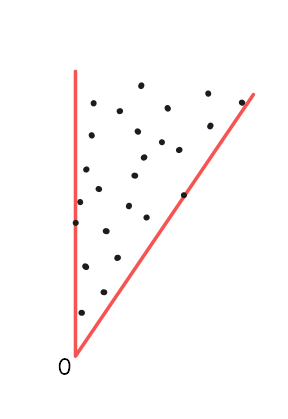
\includegraphics[width=\textwidth]{img/cone_hull.png}
        \caption{$\textbf{cone }C$}
        \label{fig:cone_hull:b}
    \end{subfigure}
     
    \caption{Kuželový obal množiny}
    \label{fig:cone_hull}
\end{figure}

\section{Nadroviny a poloprostory}

\textbf{Nadrovina} je množina ve tvaru
$$
    \left\{ x \mid a^T x = b \right\},
$$
kde $a \in \mathbb{R}^n$, $a \neq 0$ a $b \in \mathbb{R}$. Analyticky se na nadrovinu koukáme jako na množinu všech řešení netriviální lineární rovnice. Geometricky zase jako na množinu všech bodů takových, že mají konstantní skalární součin s normálovým vektorem $a$. Konstanta $b$ značí posunutí nadroviny od počátku. Nadrovinu také můžeme vyjádřit jako
$$
    \left\{ x \mid a^T (x - x_0) = 0 \right\} = x_0 + \left\{ v \mid a^T v = 0 \right\},
$$
kde $x_0$ je libovolný bod této nadroviny a $\left\{ v \mid a^T v = 0 \right\}$ je množina všech vektorů, které jsou kolmé k normálovému vektoru $a$. Nadrovina je tedy množina, která obsahuje bod $x_0$ a libovolný bod ve tvaru $x_0 + v$, kde $v$ je vektor, který je kolmý k normálovému vektoru $a$. Pro ilustraci v $\mathbb{R}^2$ viz obrázek~\ref{fig:hyperplane}.

Nadrovina dělí $\mathbb{R}^n$ na dva poloprostory. Množina 
$$
    \left\{ x \mid a^T x \leq b \right\}, \text{ resp. } \left\{ x \mid a^T x < b \right\},
$$
kde $a \neq 0$ se nazývá (uzavřený) \textbf{poloprostor}, resp. \textbf{otevřený poloprostor}. Je to tedy množina všech řešení netriviální lineární nerovnice. Podobně jako nadrovinu, můžeme poloprostor vyjádřit ve tvaru
$$
    \left\{ x \mid a^T (x - x_0) \leq 0 \right\}, \text{ resp. } \left\{ x \mid a^T (x - x_0) < 0 \right\},
$$
kde $a \neq 0$ a $x_0$ je libovolný bod z nadroviny $\left\{ x \mid a^T x = b \right\}$. Poloprostor tedy obsahuje bod $x_0$ a libovolný bod $x_0 + v$, kde $v$ je vektor, který s vnějším normálovým vektorem svírá tupý nebo pravý úhel. Tato interpretace je v $\mathbb{R}^2$ ilustrována na obrázku~\ref{fig:halfspace}. Ještě poznamenejme, že poloprostory jsou konvexní množiny, ale samozřejmě nejsou afinní.

\begin{figure}[h!]
    \centering
    \begin{subfigure}[b]{0.3\textwidth}
        \centering
        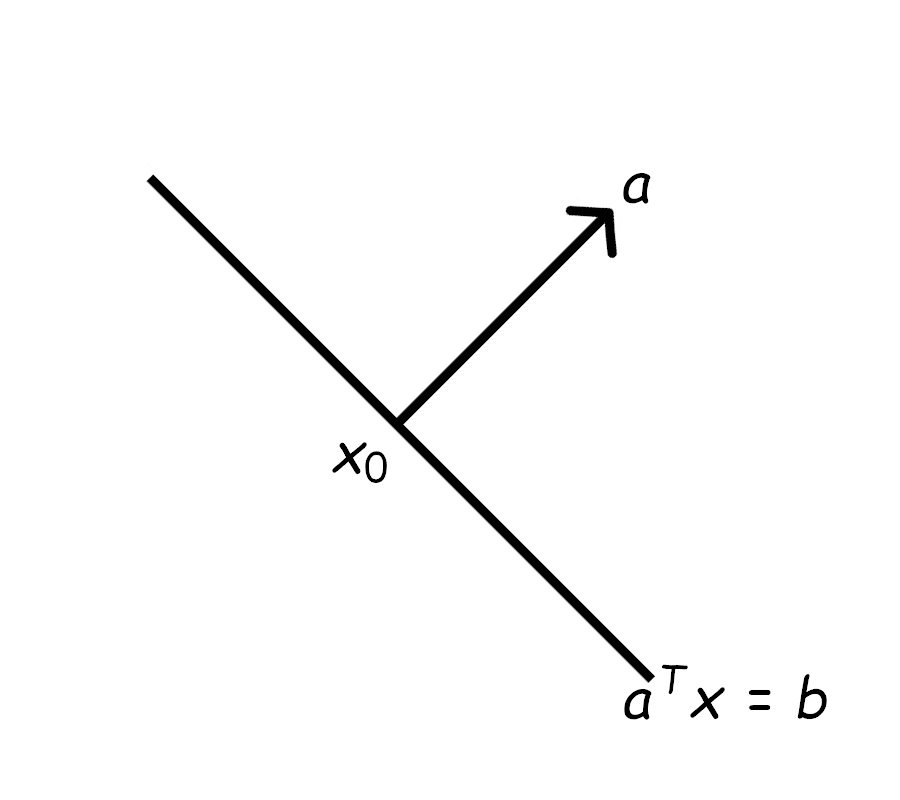
\includegraphics[width=\textwidth]{img/hyperplane.jpg}   
        \caption{Nadrovina}
        \label{fig:hyperplane}
    \end{subfigure}

    \hfill

    \begin{subfigure}[b]{0.3\textwidth}
        \centering
        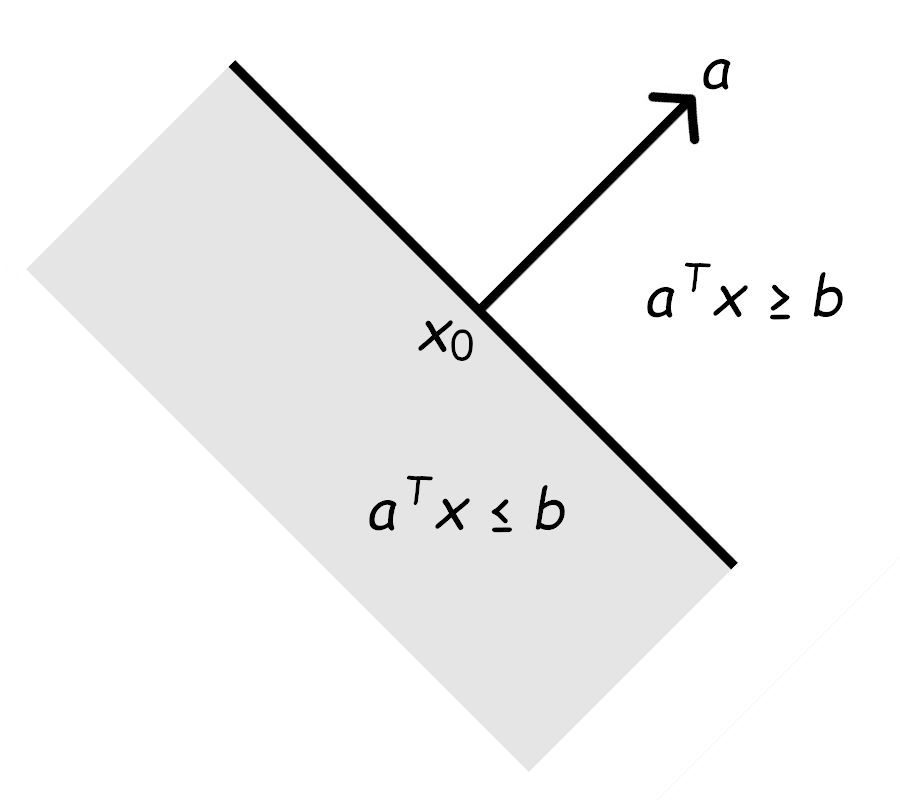
\includegraphics[width=\textwidth]{img/halfspace.jpg}   
        \caption{Poloprostor}
        \label{fig:halfspace}
    \end{subfigure}

    \caption{Nadrovina a poloprostor v $\mathbb{R}^2$.}
    \label{fig:hyperplane_halfspace}
\end{figure}

\section{Polyedry a polytopy -- PŘEPSAT / DOPLNIT}

Mějmě konečně mnoho uzavřených poloprostorů v $\mathbb{R}^n$. Množina, která vznikne jejich průnikem se nazývá \textbf{polytop}. Je-li navíc polytop omezený, potom ho nazýváme \textbf{polyedr}. Polyedr lze také ekvivalentně definovat jako konvexní obal konečně mnoha bodů v $\mathbb{R}^n$. Důležitý fakt říká Minkowského-Weyleova věta.
%Příkladem polyedrů v $\mathbb{R}^3$ jsou např. platónská tělesa, viz obrázek~\ref{fig:platon_solids}. 

\begin{vt}[Minkowski-Weyl]
    TODO
\end{vt}

%každý polytop $P$ je konečně generovaný a můžeme ho vyjadřit jako
%$$
%    P = \textbf{conv }(u_1, \dots, u_r) + \textbf{cone }(v_1, \dots, v_s),
%$$
%kde $u_i, v_i$ jsou extremální vrcholy $P$.

%\begin{figure}[h!]
%    \centering
%    \begin{subfigure}[b]{0.3\textwidth}
%        \centering
%        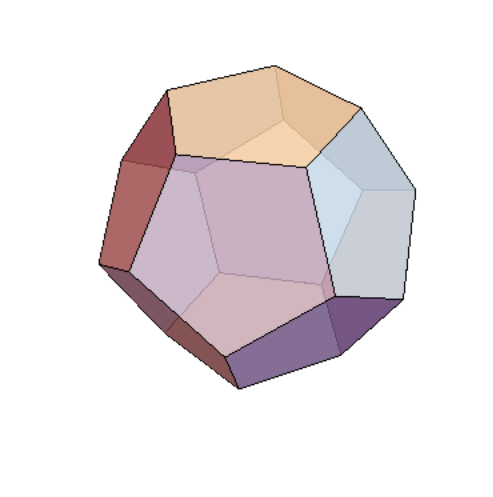
\includegraphics[width=\textwidth]{img/dodecahedron.png}   
%        \caption{Dodecahedron.}
%    \end{subfigure}
%
%    \hfill
%
%    \begin{subfigure}[b]{0.3\textwidth}
%        \centering
%        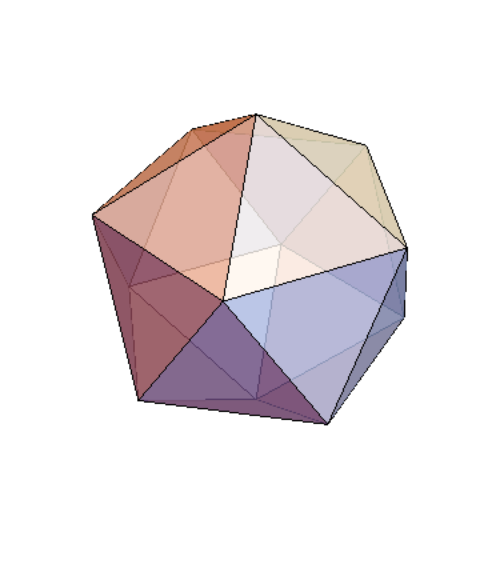
\includegraphics[width=\textwidth]{img/icosahedron.png}   
%        \caption{Icosahedron.}
%    \end{subfigure}
%
%        \begin{subfigure}[b]{0.3\textwidth}
%        \centering
%        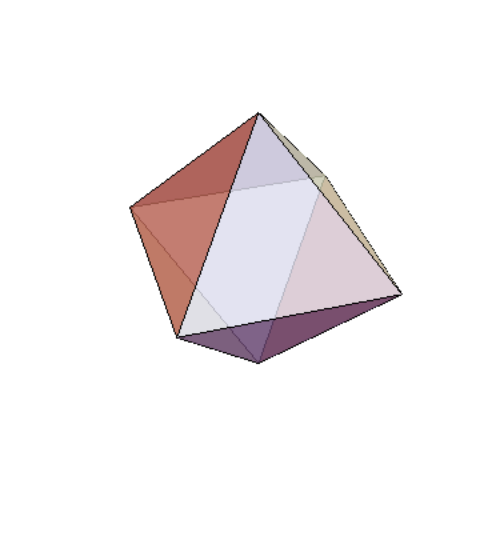
\includegraphics[width=\textwidth]{img/octahedron.png}   
%        \caption{Octahedron.}
%    \end{subfigure}
%
%    \caption{Platónská tělesa.}
%    \label{fig:platon_solids}
%\end{figure}

\chapter{Lineární programování}

\section{Formulace úlohy}

Úlohou lineárního programování rozumíme minimalizaci nebo maximalizaci lineární \textbf{účelové funkce} vzhledem k lineárním \textbf{omezením}, kde tato omezení jsou dána soustavou lineární rovnic a nerovnic. Úlohu lineárního programování lze formulovat v několika tvarech, které se liší zadáním omezení. Úloha ve \textbf{standardním tvaru} má svá omezení dána soustavou lineárních rovnic $Ax = b$. Tedy
\begin{equation}
    \min \left\{ c^T x \mid Ax = b, x \geq 0 \right\}, \tag{LP-P}
    \label{eq:LP-P}
\end{equation}
kde $A \in \mathbb{R}^{m \times n}$, $b \in \mathbb{R}^n$, $x \in \mathbb{R}^n$ a $c \in \mathbb{R}^n$. \textbf{Přípustná množina řešení} je průnikem affiního prostoru, který je definován soustavou rovnic $Ax = b$ a \textbf{nezáporného ortantu}, tj. množiny $\left\{ x \in \mathbb{R}^n \mid x_i \geq 0, i = 1, \dots, n \right\}$. Obě tyto množiny jsou konvexní a tedy i jejich průnik je rovněž konvexní množina. Dále, protože přípustnou množinu máme popsanou soustavou konečně mnoha lineárních rovnic a nerovnic, geometricky se na úlohu \ref{eq:LP-P} můžeme koukat jako na minimalizaci lineární funkce přes polyedr, který je definován touto soustavou. 

\section{Dualita}

\section{Komplementární skluzovost}

\chapter{Semidefinitní programování}

Na semidefinitní programování se můžeme koukat jako na zobecnění lineárního programování, kde proměnné jsou symetrické matice. Jedná se tedy o optimalizaci lineární funkce vzhledem k tzv. lineárním maticovým nerovnostem.

\section{Vsuvka z lineární algebry}

\subsection*{Pozitivně definitní matice}

Pracujeme s reálnými symetrickými maticemi $S = S^T$. Ty mají všechna vlastní čísla reálná a některé z nich mají zajímavou vlastnost, že všechna jejich vlastní čísla jsou kladná. Takovým maticím říkáme, že jsou pozitivně definitní. Alternativní definicí je, že matice $S$ je pozitivně definitní, jestliže $x^TSx > 0$ pro všechny nenulové vektory $x$.

\begin{pr}
$$
    x^T S x = 
    \begin{bmatrix}
        x_1 & x_2
    \end{bmatrix}
    \begin{bmatrix}
        2 & 4 \\
        4 & 9
    \end{bmatrix}
    \begin{bmatrix}
        x_1 \\
        x_2
    \end{bmatrix} =
    2 x_1^2 + 8 x_1 x_2 + 9 x_2^2
$$
Je pro všechny $x$ nenulové $x^TSx > 0$? Ano, protože můžeme výraz přepsat na součet čtverců:
$$
    x^TSx = 2 x_1^2 + 8 x_1 x_2 + 9 x_2^2 = 2 (x_1 + 2 x_2)^2 + x_2^2.
$$
TODO: obrázek kyblíčku
\end{pr}

Ukážeme si několik kritérií, jak otestovat pozitivní definitnost dané matice.

\begin{vt}
    $S = S^T$ je pozitivně definitní, jestliže lze napsat jako $S = A^T A$ pro nějakou matici $A$, která má lineárně nezávislé sloupečky.
\end{vt}
\begin{proof}
    \begin{equation}
    \label{eq:tmp}
        x^TSx = x^TA^TAx = (Ax)^T(Ax) = \lVert Ax \rVert^2 \geq 0
    \end{equation}
    $\lVert Ax \rVert^2 > 0$, jestliže sloupečky matice $A$ jsou lineárně nezávislé
\end{proof}

\begin{pr}
    $$
        S = 
        \begin{bmatrix}
            2 & 3 & 4 \\
            3 & 5 & 7 \\
            4 & 7 & 10
        \end{bmatrix} =
        \begin{bmatrix}
            1 & 1 \\
            1 & 2 \\
            1 & 3
        \end{bmatrix}
        \begin{bmatrix}
            1 & 1 & 1 \\
            1 & 2 & 3
        \end{bmatrix} =
        AA^T
    $$
    $A$ má lineárně závislé sloupečky, tj. $S$ není pozitivně definitní
\end{pr}

Dalším testem je tzv. Sylvesterovo kritérium.

\begin{vt}
    $S = S^T$ je pozitivně definitní, jestliže všechny hlavní minory $S$ jsou kladné.
\end{vt}

\begin{pr}
    $$  S =
        \begin{bmatrix}
            3 & 4 \\
            4 & 6
        \end{bmatrix},
        D_1 = 3,
        D_2 = 3 \cdot 6 - 4 \cdot 4 = 2 
    $$
    hlavní minory $D_1, D_2 > 0$; matice $S$ je pozitivně definitní 
\end{pr}

A poslední, které si uvedeme souvisí s Gaussovou eliminací.

\begin{vt}
    $S = S^T$ je pozitivně definitní, jestliže jsou všechny pivoty při Gaussově eliminaci kladné.
\end{vt}

\begin{pr}
    $$  S =
        \begin{bmatrix}
            3 & 4 \\
            4 & 6
        \end{bmatrix}
        \sim
        \begin{bmatrix}
            3 & 4 \\
            0 & \frac{2}{3}
        \end{bmatrix},
        p_1 = 3, p_2 = \frac{2}{3} 
    $$
    pivoty $p_1, p_2 > 0$; matice $S$ je pozitivně definitní
\end{pr}

\subsection*{Pozitivně semidefinitní matice}

Pro pozitivní semidefinitnost modifikujeme předcházejí definice a tvrzení pro pozitivně definitní matice následovně:
\begin{enumerate}
    \item $S = S^T$ je pozitivně semidefinitní, jestliže všechna její čísla jsou nezáporná.
    \item $S = S^T$ je pozitivně semidefinitní, jestliže $x^TSx \geq 0$ pro všechny nenulové vektory $x$.
    \item $S = S^T$ je pozitivně semidefinitní, jestliže lze napsat jako $S = A^T A$ pro nějakou matici $A$.
    \item $S = S^T$ je pozitivně semidefinitní, jestliže všechny hlavní minory $S$ jsou nezáporné.
    \item $S = S^T$ je pozitivně semidefinitní, jestliže jsou všechny pivoty při eliminaci nezáporné.
\end{enumerate}

\subsection*{Pozitivně semidefinitní kužel}

Množinu všech symetrických matic značíme $S^n$, množinu všech pozitivně semidefinitních matic značíme $S_+^n$ a množinu všech pozitivně definitních matic značíme $S_{++}^n$. 

\begin{vt}
    Množina $S_+^n$ tvoří konvexní kužel.
\end{vt}

\begin{proof}
    $\Theta_1, \Theta_2 \geq 0$, $A, B \in S_+^n$
    $$
        x^T \left( \Theta_1 A + \Theta_2 B \right) x = x^T \Theta_1 A x + x^T \Theta_2 B x \geq 0.
    $$
\end{proof}

Množině $S_+^n$ se říká pozitivně semidefinitní kužel.

\noindent\textbf{??chci ukázat i uzavřenost a další vlastnosti, jak se česky řekne proper cone??}

\subsection*{Spektraedry}

Definujeme tzv. L\"{o}wnerovo částečné uspořádání
$$
    A \succeq B \iff A - B \in S_+^n.
$$

\begin{df}
    Lineární maticová nerovnost (LMI) je ve tvaru
    $$
        A_0 + \sum_{i=1}^n A_i x_i \succeq 0,
    $$
    kde $A_i \in S^n$.
\end{df}

\begin{df}
    Říkáme, že $S \subset \mathbb{R}^n$ je spektraedr, jestliže lze napsat ve tvaru
    $$
        S = \left\{ (x_1, \dots, x_m) \in \mathbb{R}^m \mid A_0 + \sum_{i=1}^m A_i x_i \succeq 0 \right\}
    $$
    pro nějaké symetrické matice $A_0, \dots, A_m \in S^n$.
\end{df}

Spektraedr je tedy množina, která je definována konečným počtem LMI. Můžeme si všimnout analogie s definicí polyedru, který je přípustnou množinu pro lineární program. Podobně spektraedr je přípustnou množinou pro semidefinitní program.

Geometricky je spektraedr definován jako průnik pozitivně semidefinitního kuželu $S_+^n$ a afinního podprostoru $\textbf{span}\left\{ A_1, \dots, A_m \right\}$ posunutého do $A_0$.

Spektraedry jsou uzavřené množiny, neboť LMI je ekvivalentní nekonečně mnoha skalárních nerovností ve tvaru $v^T(A_0 + \sum_{i=1}^m A_ix_i)v \geq 0$, jednu pro každou hodnotu $v \in \mathbb{R}^n$.

Vždy můžeme několik LMI \uv{scucnout} do jedné. Stačí zvolit matice $A_i$ blokově diagonální. Odtud snadno vídíme, že polyedr je speciálním případem spektraedru. Polyedr bude mít všechny matice $A_i$ diagonální.

\begin{pr}
    $$
        \left\{ (x, y) \in \mathbb{R}^2 \mid A(x,y) =
        \begin{bmatrix}
            x + 1 & 0      & y \\
            0     & 2      & -x - 1 \\
            y     & -x - 1 & 2
        \end{bmatrix}
        \succeq 0 \right\}
    $$
\end{pr}

\section{Primární úloha}

Semidefinitní program je lineární optimalizační problém přes spektraedr. Primární úlohu ve standardním tvaru můžeme napsat jako:
\begin{equation}\tag{SDP-P}
    \min \left\{ \langle C, X \rangle \mid \langle A_i, X \rangle = b_i, i=1, \dots, m; X \succeq 0 \right\},
    \label{eq:SDP-P}
\end{equation}
kde $C, A_i \in S^n$, $\langle X, Y \rangle = \textbf{Tr}(X^T Y) = \sum_{ij} X_{ij}Y_{ij}$ a $X \in S^n$ je proměnná, nad kterou provádíme minimalizaci.

\begin{pr}
    $$
        \min \left\{
            \left\langle
            \begin{bmatrix}
                2 & 1 \\
                1 & 0
            \end{bmatrix},
            \begin{bmatrix}
                x_{11} & x_{12} \\
                x_{12} & x_{22}
            \end{bmatrix}
            \right\rangle \middle|
            \left\langle
            \begin{bmatrix}
                1 & 0 \\
                0 & 1
            \end{bmatrix},
            \begin{bmatrix}
                x_{11} & x_{12} \\
                x_{12} & x_{22}
            \end{bmatrix}
            \right\rangle = 1,
            \begin{bmatrix}
                x_{11} & x_{12} \\
                x_{12} & x_{22}
            \end{bmatrix} \succeq 0
        \right\}
    $$
    Po úpravě:
    $$
        \min \left\{
            2 x_{11} + 2 x_{12} \middle| x_{11} + x_{22} = 1, 
            \begin{bmatrix}
                x_{11} & x_{12} \\
                x_{12} & x_{22}
            \end{bmatrix} \succeq 0
        \right\}.
    $$
    Jak vypadá přípustná množina? Použijeme Sylvesterovo kritérium, tj.
    $$
        x_{11} \geq 0, x_{11} x_{22} - x_{12}^2 \geq 0.
    $$
    Z LMI vyjádříme $x_{22}$, tj.
    $$
        x_{22} = 1 - x_{11}
    $$
    Dosadíme do přechozího a dostaneme
    $$
        x_{11} \geq 0, x_{11} \left(1 - x_{11}\right) - x_{12}^2 \geq 0
    $$
    Po úpravě
    $$
        x_{11} \geq 0, \left(x_{11} - \frac{1}{2}\right)^2 + x_{12}^2 \leq \frac{1}{4}
    $$
    Vidíme tedy, že přípustná množina (zobrazena na obrázku~TODO) je kruh s poloměrem $\frac{1}{2}$ a se středem v bodě $(x_{11}, x_{12}) = (\frac{1}{2}, 0)$. Řešením úlohy je matice
    $$
        X^* \approx
        \begin{bmatrix}
            0.1464  & -0.3536 \\
            -0.3536 &  0.8536
        \end{bmatrix}
    $$
    s cenou $\approx -0.4142$. Implementace v softwaru MOSEK: \url{https://github.com/c0n73x7/D1PL0MK4/blob/master/mosek/ex3.py}.

    \noindent \textbf{TODO: obrázek přípustné množiny s optimálním řešením z mosek implementace}
\end{pr}

\section{Dualita}

$$
    \max \left\{ b^Ty \ \middle|\ \sum_{i=1}^m A_i y_i \preceq C \right\},
$$
kde $b = (b_1, \dots, b_m)$ a $y = (y_1, \dots, y_m)$ jsou duální proměnné.

Vztah mezi primární a duální úlohou je podobně jako u lineárního programování v tom, že řešení jedné úlohy lze použít jako odhad na úlohu druhou. Nechť $X$ je libovolné přípustné řešení primární úlohy a $y$ je libovolné přípustné řešení duální úlohy. Potom
$$
    \langle C, X \rangle - b^T y =
    \langle C, X \rangle - \sum_{i=1}^m y_i \langle A_i, X \rangle =
    \left\langle C - \sum_{i=1}^m A_i y_i, X \right\rangle \geq 0
$$


\section*{WIP}
\subsection*{Odvození duální úlohy}

\noindent Lagrangeovo funkce
$$
    L(X, \lambda, Z) = \langle C, X \rangle - \sum_{i=1}^m \lambda_i \left( \langle A_i, X \rangle - b_i \right) - \langle Z, X \rangle
$$

\noindent primární úloha odpovídá
$$
    \min_{X \in S^n} \max_{\lambda \in \mathbb{R}^m, Z \succeq 0} L(X, \lambda, Z)
$$

\noindent z Lagrangeovy duality
$$
    g(\lambda, Z) = \inf_{X \in S^n} L(X, \lambda, Z) = 
    \begin{cases}
        \lambda^T b & \dots\ C - \sum_{i=1}^m \lambda_i A_i - Z = 0, \\
        -\infty     & \dots\ \text{jinak.}
    \end{cases}
$$

\noindent eliminujeme $Z$
$$
    \sup \left\{ b^T \lambda\ \middle|\ \sum_{i=1}^m A_i \lambda_i \preceq C \right\}
$$






Stopa matice $A \in R^{n \times n}$ je $\textbf{Tr}(A) = \sum_{i=1}^n A_{ii}$.

\begin{vt}
$S, T$ jsou pozitivně definitní $\implies$ $S + T$ je pozitivně definitní
\end{vt}

\begin{proof}
$x^T (S+T) x = x^T S x + x^T T x > 0$
\end{proof}


Úlohy s racionálními daty nemusí mít racionální optimální řešení.


\noindent Lagrangovo funkce a dualita konvexního programování (příloha?);

\noindent z toho dualitu semidefinitního programování;

\noindent rozdíl oproti lineárnímu programování;

\noindent příklad

\subsection*{Relaxace}
\noindent vektorové programování

%spektraedr, formulace, dualita, semidefinitní kužel, duální kužel, ...
%vektorové programování a jeho ekvivalence, formulace úloh

\clearpage


% ------------------------- ČÁST: KOMBINATORICKÉ ÚLOHY ----------------------- %
\part{Kombinatorické úlohy}

\chapter{Shannonova kapacita}

Představme si zašuměný komunikační kanál, kterým posíláme zprávy, které jsou složeny ze symbolů (písmen) nějaké konečné abecedy. Vlivem šumu mohou být některé symboly špatně interpretovány a naším cílem je vybrat co největší počet slov délky $k$ tak, aby žádná dvě slova nebyla vlivem šumu zaměnitelná.

Problém si formalizujeme v řeči teorie grafů. Mějme neorientovaný graf $G = (V, E)$, kde množina vrcholů představuje symboly z konečné abecedy a dva vrcholy $x, y$ jsou spojeny hranou, pokud vrchol $x$ může být vlivem šumu zaměněn za $y$.

Maximální počet nezaměnitelných zpráv délky $1$ je roven $\alpha(G)$, kde $\alpha(G)$ značí velikost největší nezávislé množiny v grafu $G$. Pro popis delších zpráv definujeme \textbf{silný součin} $G \cdot H$ grafů $G$ a $H$ následovně:
$$
    V(G \cdot H) = V(G) \times V(H),
$$
\begin{equation*}
    \begin{split}
    E(G \cdot H) = &\left\{ (i,u)(j,v) \mid ij \in E(G) \wedge uv \in E(H) \right\} \cup \\
                   &\left\{ (i,u)(j,v) \mid ij \in E(G) \wedge u = v \right\} \cup \\
                   &\left\{ (i,u)(j,v) \mid i = j \wedge uv \in E(H) \right\}.
    \end{split}
\end{equation*}

\begin{pr}
Pro graf $P_4 = a-b-c-d-e$ je silný součin $P_4 \cdot P_4$ zobrazen na obrázku~\ref{fig:strong_product_P4_P4}. Z obrázku je hezky vidět, že např. zpráva $cd$ (na obrázku červeně) může být zaměněna s $bc$, $bd$, $be$, $cc$, $ce$, $dc$, $dd$ a $de$ (na obrázku oranžově). Podobně pro další zprávy.
\end{pr}

\begin{figure}[h!]
    \centering
    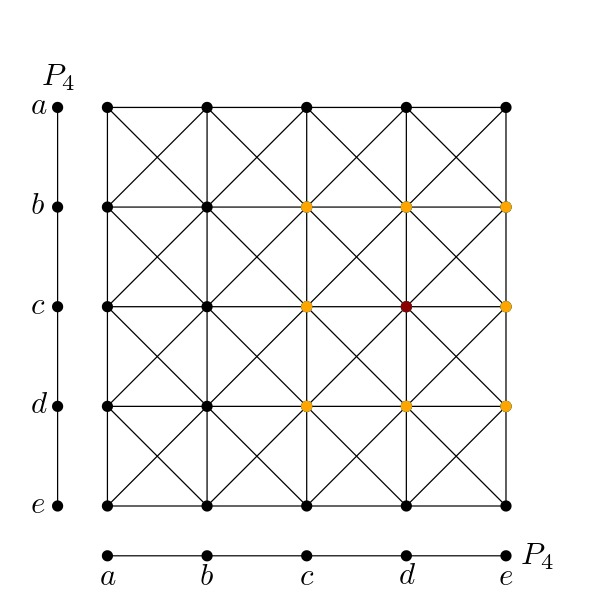
\includegraphics[width=0.5\textwidth]{img/strong_product_P4_P4.png}   
    \caption{$P_4 \cdot P_4$}
    \label{fig:strong_product_P4_P4}
\end{figure}

Pro jednoduchost budeme silný součin $k$ kopií grafu $G$ značit $G^k$. Tedy $\alpha(G^k)$ je maximální počet nezaměnitelných zpráv délky $k$. \textbf{Shannonova kapacita} grafu $G$ je definována jako
$$
    \Theta(G) = \sup \left\{ \alpha(G^k)^{1/k} \mid k = 1, 2, \dots \right\}.
$$

Neví se, zda pro libovolný graf $G$ existuje vůběc nějaký algoritmus, kterým bychom určili hodnotu $\Theta(G)$. Přesto je alespoň něco známo. Pro perfektní grafy Claude E. Shannon ukázal, že $\Theta(G) = \alpha(G)$. To také znamená, že pro perfektní grafy lze $\Theta(G)$ určit v polynomiálním čase. Dalším kdo se problémem zabýval byl László Lovász, který velmi hezkým způsobem ukázal, že kružnice délky $5$ má kapacitu $\sqrt{5}$. Na Lovászův postup se dále podíváme, protože vede k obecnému hornímu odhadu na $\Theta(G)$.

\section{$\Theta(C_5) = \sqrt{5}$}

\textbf{Tenzorový součin} vektorů $\mathbf{u} = \left(u_1, \dots, u_n \right)$ a $\mathbf{v} = \left(v_1, \dots, v_m \right)$ je
$$
    \mathbf{u} \circ \mathbf{v} = \left( u_1 v_1, \dots, u_1 v_m, u_2 v_1, \dots, u_n v_m \right).
$$

Užitečné bude následující pozorování, které dává do souvisloti skalární a tenzorový součin.

\begin{pz}
    Nechť $\mathbf{x}, \mathbf{u}$ jsou vektory délky $n$ a $\mathbf{y}, \mathbf{v}$ jsou vektory délky $m$. Potom platí
    \begin{equation}
        \left( x \circ y \right)^T \left( u \circ v \right) = \left( x^T u \right) \left( y^T v \right).
        \label{eq:tensor_scalar_product}
    \end{equation}
\end{pz}

\begin{proof}
    Levá strana:
    \begin{equation*}
        \begin{split}
        & \left(x_1 y_1, x_1 y_2, \dots, x_1 y_m, \dots, x_n y_m \right)^T \left( u_1 v_1, u_1 v_2, \dots, u_1 v_m, \dots, u_n v_m \right) = \\
        & x_1 y_1 u_1 v_1 + x_1 y_2 u_1 v_2 + \dots + x_1 y_m u_1 v_m + \dots + x_m y_m u_n v_m
        \end{split}
    \end{equation*}
    Pravá strana:
    \begin{equation*}
        \begin{split}
            & \left( x_1 u_1 + \dots + x_n u_n \right) \cdot \left( y_1 v_1 + \dots + y_n v_m \right) = \\
            & x_1 y_1 u_1 v_1 + x_1 y_2 u_1 v_2 + \dots + x_1 y_m u_1 v_m + \dots + x_m y_m u_n v_m
        \end{split}
    \end{equation*}
\end{proof}

Mějme graf $G = (V,E)$, kde $V = \left\{ 1, \dots, n \right\}$. Systém $\left( \textbf{v}_1, \dots, \textbf{v}_n \right)$ jednotkových vektorů v Euklidovském prostoru takový, že
$$
    \forall ij \notin E \implies \textbf{v}_i \perp \textbf{v}_j
$$
nazýváme \textbf{ortonormální reprezentace} grafu $G$. Poznamenejme, že každý graf má nějakou ortonormální reprezentaci, např. $1 \mapsto \mathbf{e}_1, \dots, n \mapsto \mathbf{e}_n$.

\begin{lm}
    Nechť $\left( \mathbf{u}_1, \dots, \mathbf{u}_n \right)$ je ortonormální reprezentace grafu $G$ a $\left( \mathbf{v}_1, \dots, \mathbf{v}_m \right)$ je ortonormální reprezentace grafu $H$. Potom $\mathbf{u}_i \circ \mathbf{v}_j$ je ortonormální reprezentace grafu $G \cdot H$.
\end{lm}

\begin{proof}
    Použijeme vztah \ref{eq:tensor_scalar_product}. $\left( u_i \circ v_j \right)^T \left( u_k \circ v_l \right) = \left( u_i^T u_k \right) \left( v_j^T v_l \right) = 0 \iff ik \notin E(G) \vee jl \notin E(H)$.
\end{proof}

\begin{figure}[h!]
    \centering
    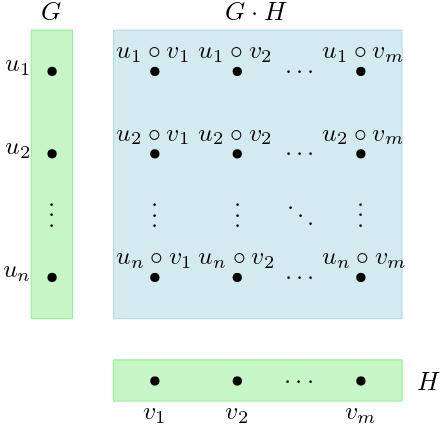
\includegraphics[width=0.5\textwidth]{img/shannon_lemma.png}   
    \caption{Ortornomální reprezentace $G \cdot H$.}
    \label{fig:orthonormal_repr_GH}
\end{figure}

\textbf{Hodnotu} ortonormální reprezentace $\left(u_+, \dots, u_n \right)$ definujeme jako:
$$
    \min_c \max_{i = 1, \dots, n} \frac{1}{\left( c^T u_i \right)^2}.
$$
Vektoru $c$, pro který nastává minimum říkáme \textbf{handle} dané ortonormální reprezentace.

Dále definujeme funkci $\vartheta(G)$ jako minimální hodnotu přes všechny ortonormální reprezentace grafu $G$. Ortonormální reprezentaci, pro kterou nastává minumum nazýváme \textbf{optimální}.

Funkci $\vartheta(G)$ se říká \textbf{Lovászova theta funkce} a ona je právě již zmíněným horním odhadem na $\Theta(G)$. Podívejme se na některé její vlastnosti.

\begin{lm}
    $\vartheta(G \cdot H) \leq \vartheta(G) \vartheta(H)$
\end{lm}

\begin{proof}
    Nechť $\left( u_1, \dots, u_n \right)$ je optimální ortonormální reprezentace grafu $G$ s \uv{rukojetí} $c$ a $\left( v_1, \dots, v_m \right)$ je optimální ortonormální reprezentace grafu $H$ s \uv{rukojetí} $d$. Pak $c \circ d$ je jednotkový vektor a platí:
    $$
        \vartheta(G \cdot H) \leq \max_{i,j} \frac{1}{\left( \left( c \circ d \right)^T \left( u_i \circ v_j \right) \right)^2} = \max_i \frac{1}{\left( c^T u_i \right)^2} \cdot \max_j \frac{1}{\left( d^T v_j \right)^2} = \vartheta(G)\vartheta(H).
    $$
\end{proof}

\begin{lm}
    $\alpha(G) \leq \vartheta(G)$
\end{lm}

\begin{proof}
    TODO (máš to někde na papíře)
\end{proof}

\begin{lm}
    $\Theta(G) \leq \vartheta(G)$
\end{lm}

\begin{proof}
    TODO (máš to někde na papíře)
\end{proof}

\begin{vt}
    $\Theta(C_5) = \sqrt{5}$
\end{vt}

\begin{proof}
    TODO (obě nerovnosti, obrázek, spherical cosine theorem)
\end{proof}


\section{Další vlastnosti $\vartheta(G)$}
vztah k barvení ($\overline{G}$), ...


\section{Semidefinitní program pro $\vartheta(G)$}

formulace semidefinitních programů (jsou dva ekvivalentní -- to asi nenaimplementuješ, je to docela pekelný, nic nespočítáš), subgradientní aproximační metoda (zkusit naimplementovat???)


\chapter{Problém maximálníhu řezu}

formulace úlohy, approximační algoritmy, porovnání semidefinitních programů..

\chapter{Problém obchodního cestujícího}


\clearpage


% ---------------------------------- Závěr ----------------------------------- %
\chapter*{Závěr}
\addcontentsline{toc}{chapter}{Závěr}

V prvních čtyřech kapitolách je shrnuta teorie, která se dále využívá při popisu úloh kombinatorické optimalizace.

V kapitole o Shannonově kapacitě se věnujeme Lovászově $\vartheta$ funkci a jejímu využití. Byly naimplementovány a následně porovnány dva modely s přesnou hodnotou pro liché kružnice. Jednodušší model, který dává rovnou hodnotu $\vartheta$ funkce byl přesnější. U druhého modelu, ze kterého dostaneme hodnotu $1/\sqrt{\vartheta}$, byly patrné chyby už pro malé grafy. Problémem je, že úloha není ve standardním tvaru a frameworky typu Mosek jsou optimalizovány hlavně na práci s úlohami ve standardním tvaru. Dále byl puštěn výpočet pro vylepšení dolního odhadu Shannonovy kapacity kružnice $C_7$, ale nezávislá množina, která by odhad vylepšila se nenašla.

Pro úlohu MAX $k$-CUT byly pro účely testování implementovány čtyři algoritmy a pro úlohu kapacitního MAX $k$-CUTu další dva. U experimentu pro úlohu MAX $3$-CUT vyšel nejhůře algoritmus~\ref{alg:gw-max-3-cut}, který má nejlepší aproximační poměr, což je to dáno složitostí modelu založeného na komplexním semidefinitním programování, který je třikrát větší než model použitý v ostatních algoritmech a navíc obsahuje hodně omezení (vznikaly zaokrouhlovací chyby). Pro MAX $4$-CUT a MAX $5$-CUT vyšel nejlépe algoritmus~\ref{alg:n-max-k-cut-2}, který je jen navrhnut v závěru článku \cite{newman} a není pro něj znám aproximační poměr. U~kapacitní verze byly porovnány dva přístupy: algoritmus založený na lokálním prohledávání a náš algoritmus využívající semidefinitní programování. Oba algoritmy dávaly srovnatelné výsledky, ale rozdíl byl hlavně v době běhu, kde jasně vyhrává algoritmus využívající lokální prohledávání. Algoritmus založený na semidefinitní programování dával lepší výsledky, když součet kapacit jednotlivých množin byl větší než počet vrcholů grafu. 

Dále by mohla být věnována pozornost analýze algoritmu~\ref{alg:n-max-k-cut-2}, o kterém není známé nic.

Celá práce i s implementacemi je dostupná na \url{https://github.com/c0n73x7/D1PL0MK4}.

\clearpage


% ---------------------------- Použitá literatura ---------------------------- %
\bibliography{citace}
\bibliographystyle{plain}

\end{document}
